\section{Particle picking}
 \begin{figure}[H]
  \centering
  \captionsetup{width=.8\linewidth} 
  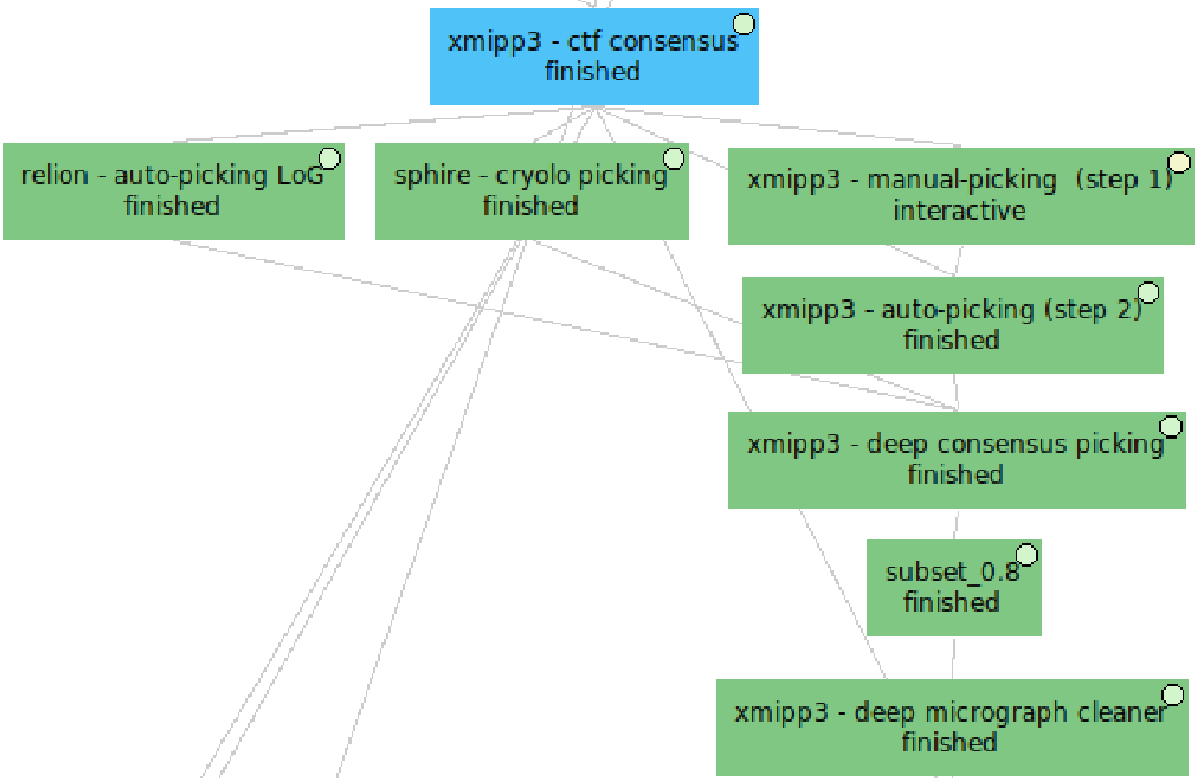
\includegraphics[width=0.75\textwidth]
  {{images/workflow_3.pdf}}
  \caption{Particle picking workflow (Green color).}
  \label{fig:workflow_3}
  \end{figure}

Since the reconstruction of the 3D density map of the macromolecule is based on images of individual single particles, the next step is essential in the image processing workflow. With the particle picking step we will retrieve the coordinates of each single particle.\\

Because manual picking can be very tedious, some tools have been designed to help in this task. We have integrated in \scipion different picking tools that can be  used individually or in combination to obtain the final coordinates. Currently, we have tools available from \ttt{Eman2}, \ttt{Relion}, \ttt{Bsoft}, \ttt{Sphire} and \ttt{Xmipp}. In this tutorial we are going to use three different protocols that integrate tools from \ttt{Relion} (\scommand{relion- auto-picking LoG} \citep{relion32018}), \ttt{Sphire} (\scommand{sphire-cryolo picking} \citep{cryolo2019}) and \ttt{Xmipp} (\scommand{xmipp3- manual-picking (step1)} and \scommand{xmipp3- auto-picking (step 2)} \citep{sorzano2013semiautomatic}).\\

The protocol \scommand{relion- auto-picking LoG} (\ffigure{fig:relion_autopicking}) provides particle coordinates in an automatic way. Together with the 47 input micrographs and the size in pixels for each particle, the protocol form allows to set specific parameters to compute the Laplacian of Gaussian (LoG).\\
\begin{figure}[H]
  \centering
  \captionsetup{width=.8\linewidth} 
  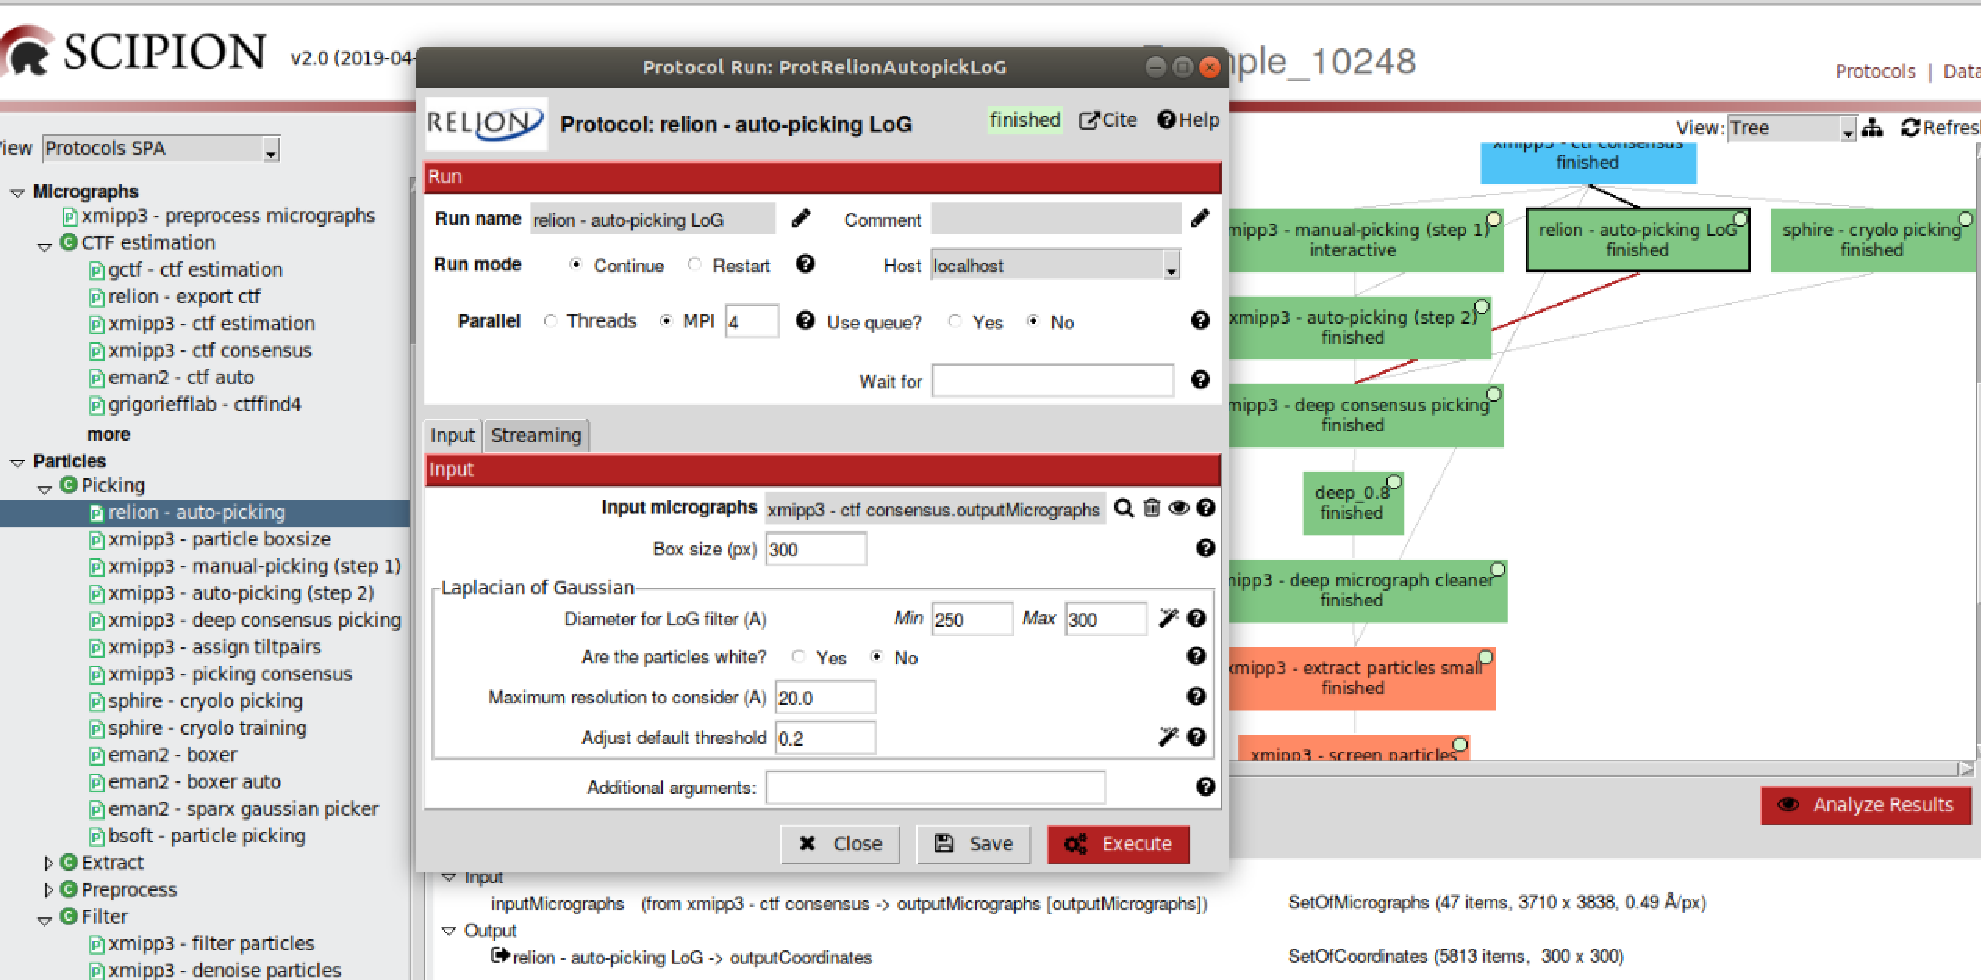
\includegraphics[width=0.95\textwidth]
  {{images/relion_autopicking.pdf}}
  \caption{Filling in the protocol \scommand{relion- auto-picking LoG}.}
  \label{fig:relion_autopicking}
  \end{figure}
The protocol \scommand{sphire-cryolo picking} (\ffigure{fig:sphire-cryolo}) integrates a fully automated particle picker based on deep learning. The protocol form also requires the 47 micrographs and the size of particles, and gives you the possibility of using your own network model, obtained in a previous training step, instead the general one. \ttt{Confidence threshold} allows to perform a more or less conservative picking by increasing or decreasing the value of this param.\\
\begin{figure}[H]
  \centering
  \captionsetup{width=.8\linewidth} 
  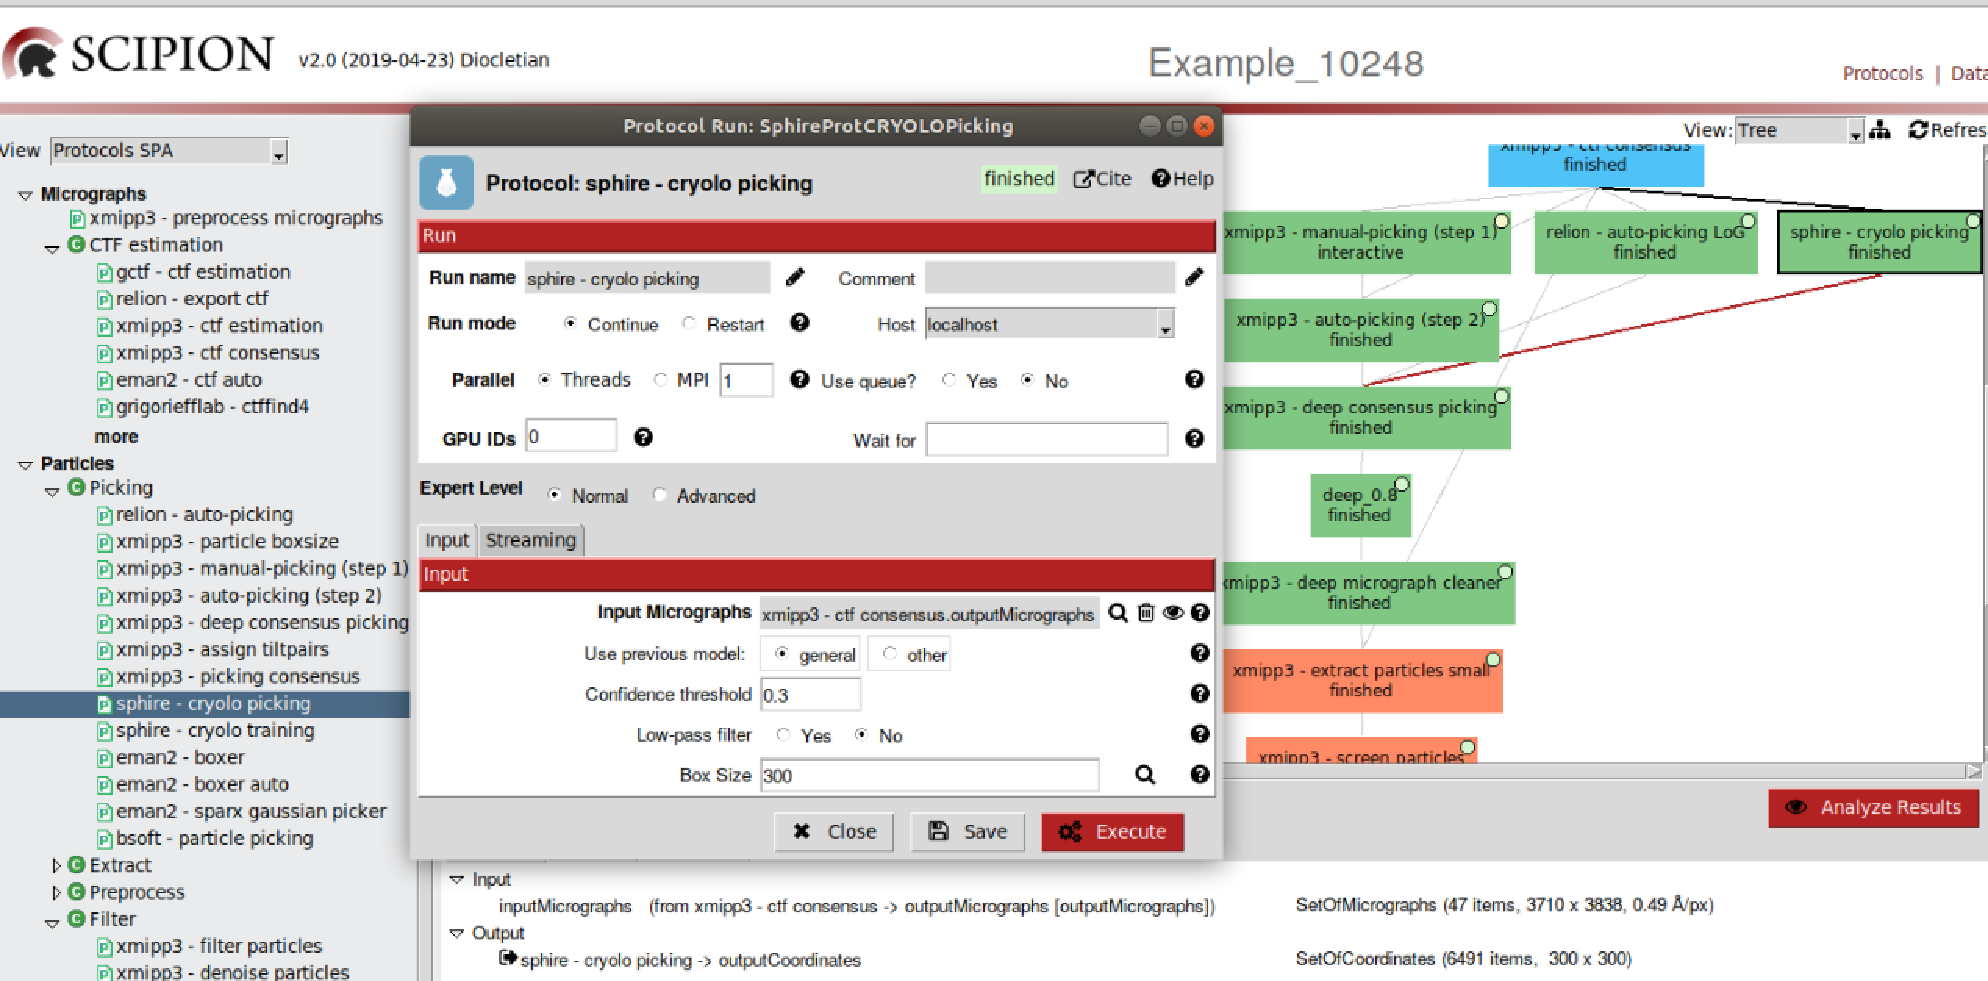
\includegraphics[width=0.95\textwidth]
  {{images/sphire_cryolo.pdf}}
  \caption{Completing in the protocol \scommand{sphire-cryolo picking}.}
  \label{fig:sphire-cryolo}
  \end{figure}
The protocol \scommand{xmipp3- manual-picking (step1)} (\ffigure{fig:xmipp_manual_picking_step1}) is the firt part of the \ttt{Xmipp} picking method, and allows to perform manual picking in a set of micrographs either manually or in a supervised mode. This protocol only requires as input the set of micrographs.\\
\begin{figure}[H]
  \centering
  \captionsetup{width=.8\linewidth} 
  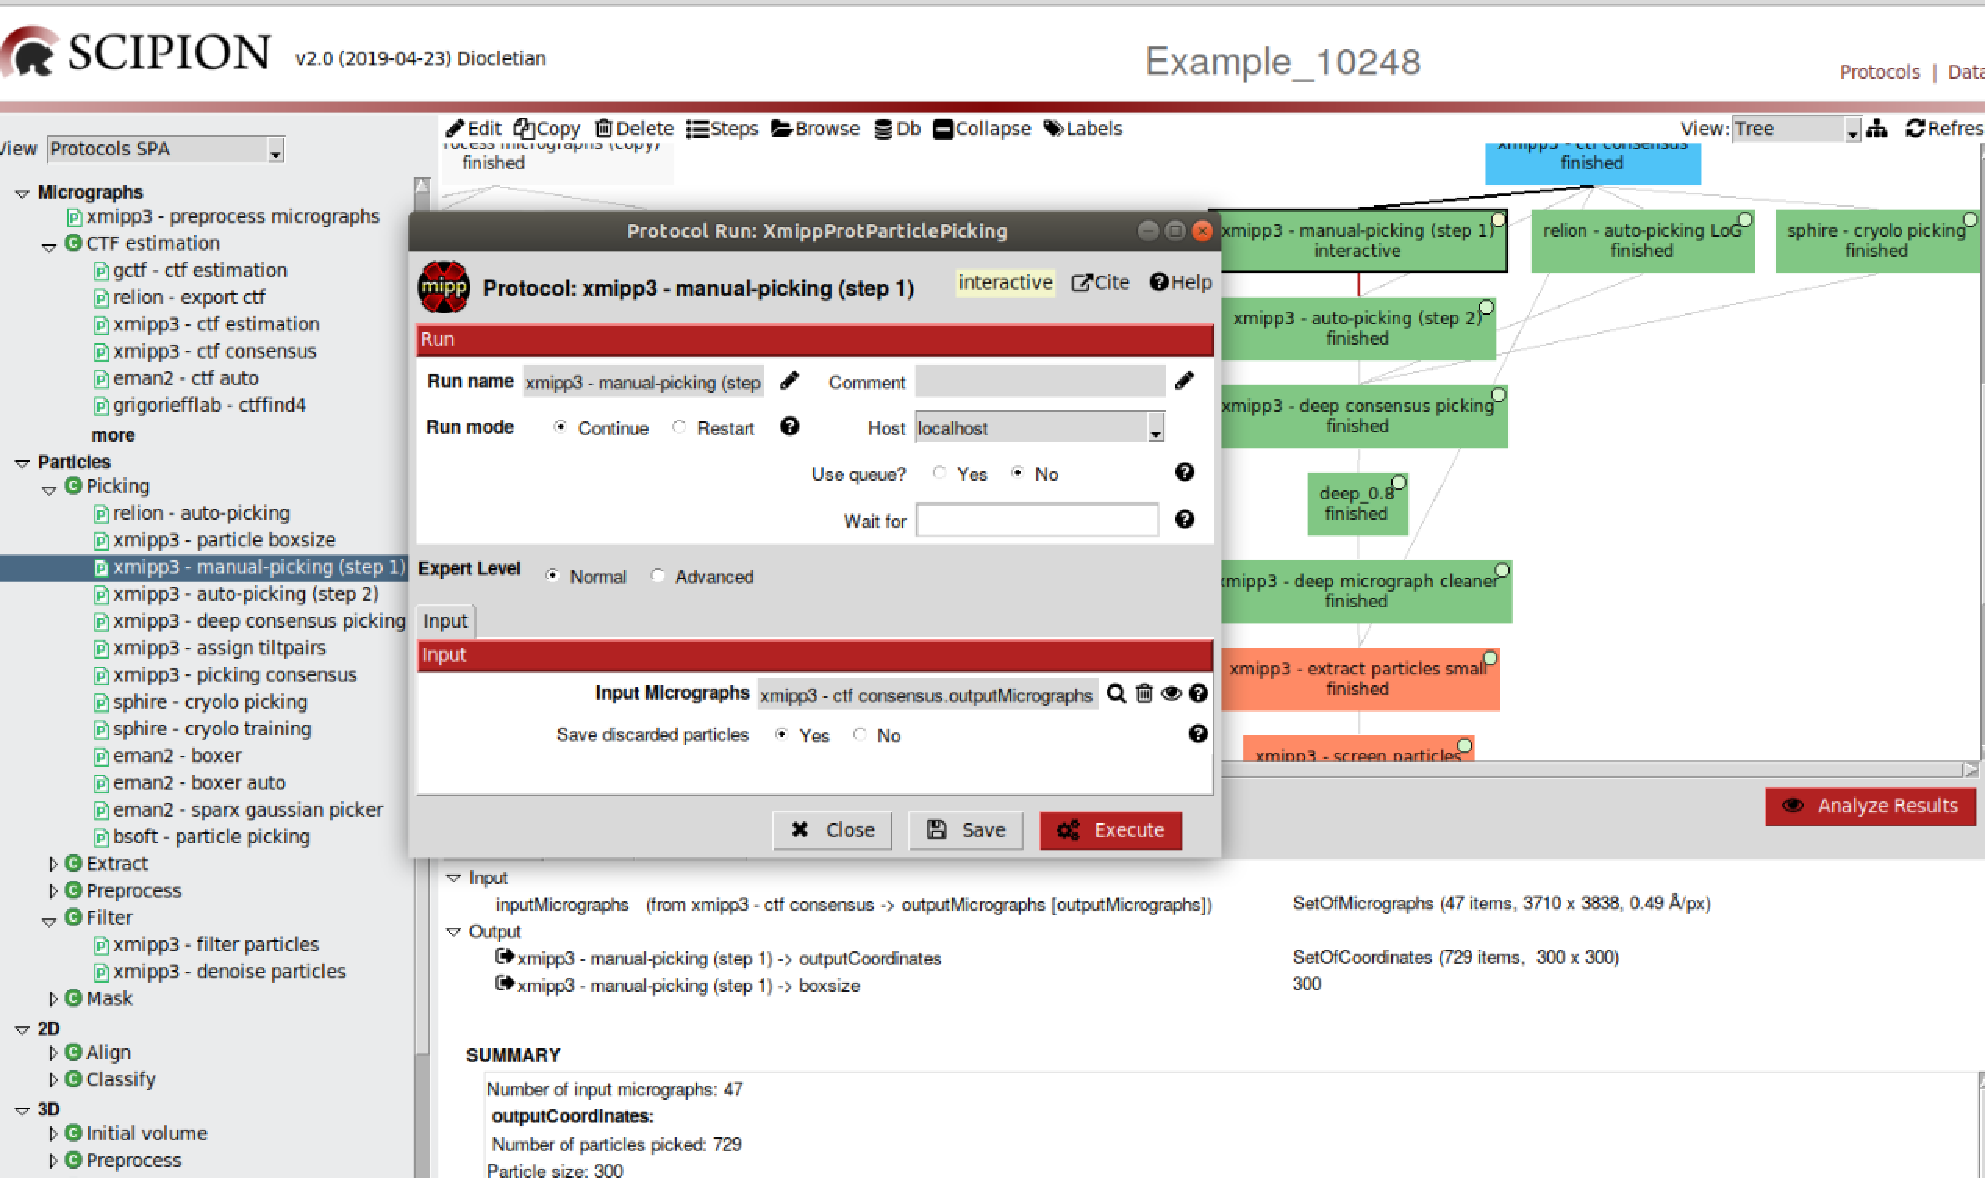
\includegraphics[width=0.95\textwidth]
  {{images/xmipp_manual_picking_step1.pdf}}
  \caption{Filling in the protocol \scommand{xmipp3- manual-picking (step1)}.}
  \label{fig:xmipp_manual_picking_step1}
  \end{figure}
  After executing this protocol, the respective box will become light yellow because an interactive job is running and it can be relaunched at any time.\\
  
  The \ttt{Xmipp} picking GUI contains a control panel with the list of micrographs and some other parameters. The micrograph that we are going to pick is displayed in a separate window and we can apply to it a number of filters/enhancements (like Gaussian blurring, Invert contrast, adjust histogram, etc.) just to improve the visualization of particles. Main control actions are:
  \begin{itemize}
   \item \ttt{Shift} + \ttt{Mouse wheel}: Zoom in and out of the overview window.
   \item \ttt{Mouse left} botton: Mark particles. You may move its position by clicking the left mouse button on the selected particle and dragging it to a new position.
   \item \ttt{Shift} + \ttt{Mouse left}: Remove a selected particle.
   \item You can apply filters in the micrographs to see the particles better. Select those filters in the menu \ttt{Filters}. 
  \end{itemize}

  In the manual/supervised step, we start picking manually a few of micrographs (5 in this case) and then clik the \ttt{Active training} button. At this point, the program will train a classifier based on machine learning and will propose some coordinates automatically. You can ``correct'' the proposal of the classifier by adding missing particles or removing wrongly picked ones. After training with a few more micrographs, we can register the output coordinates by clicking the \ttt{Coordinates} red button.\\
  
  After manual picking, we can close the GUI and open the protocol \scommand{xmipp3- auto-picking (step 2)} (\ffigure{fig:xmipp_autopicking_step2}). Select as inputs the previous manual/supervised execution and all micrographs (\ttt{Micrographs to pick}: \ttt{Other}). The method will pick the rest of micrographs automatically. At the end, we can review the picking coordinates and we still have the chance to add/remove particles.
  
  \begin{figure}[H]
  \centering
  \captionsetup{width=.8\linewidth} 
  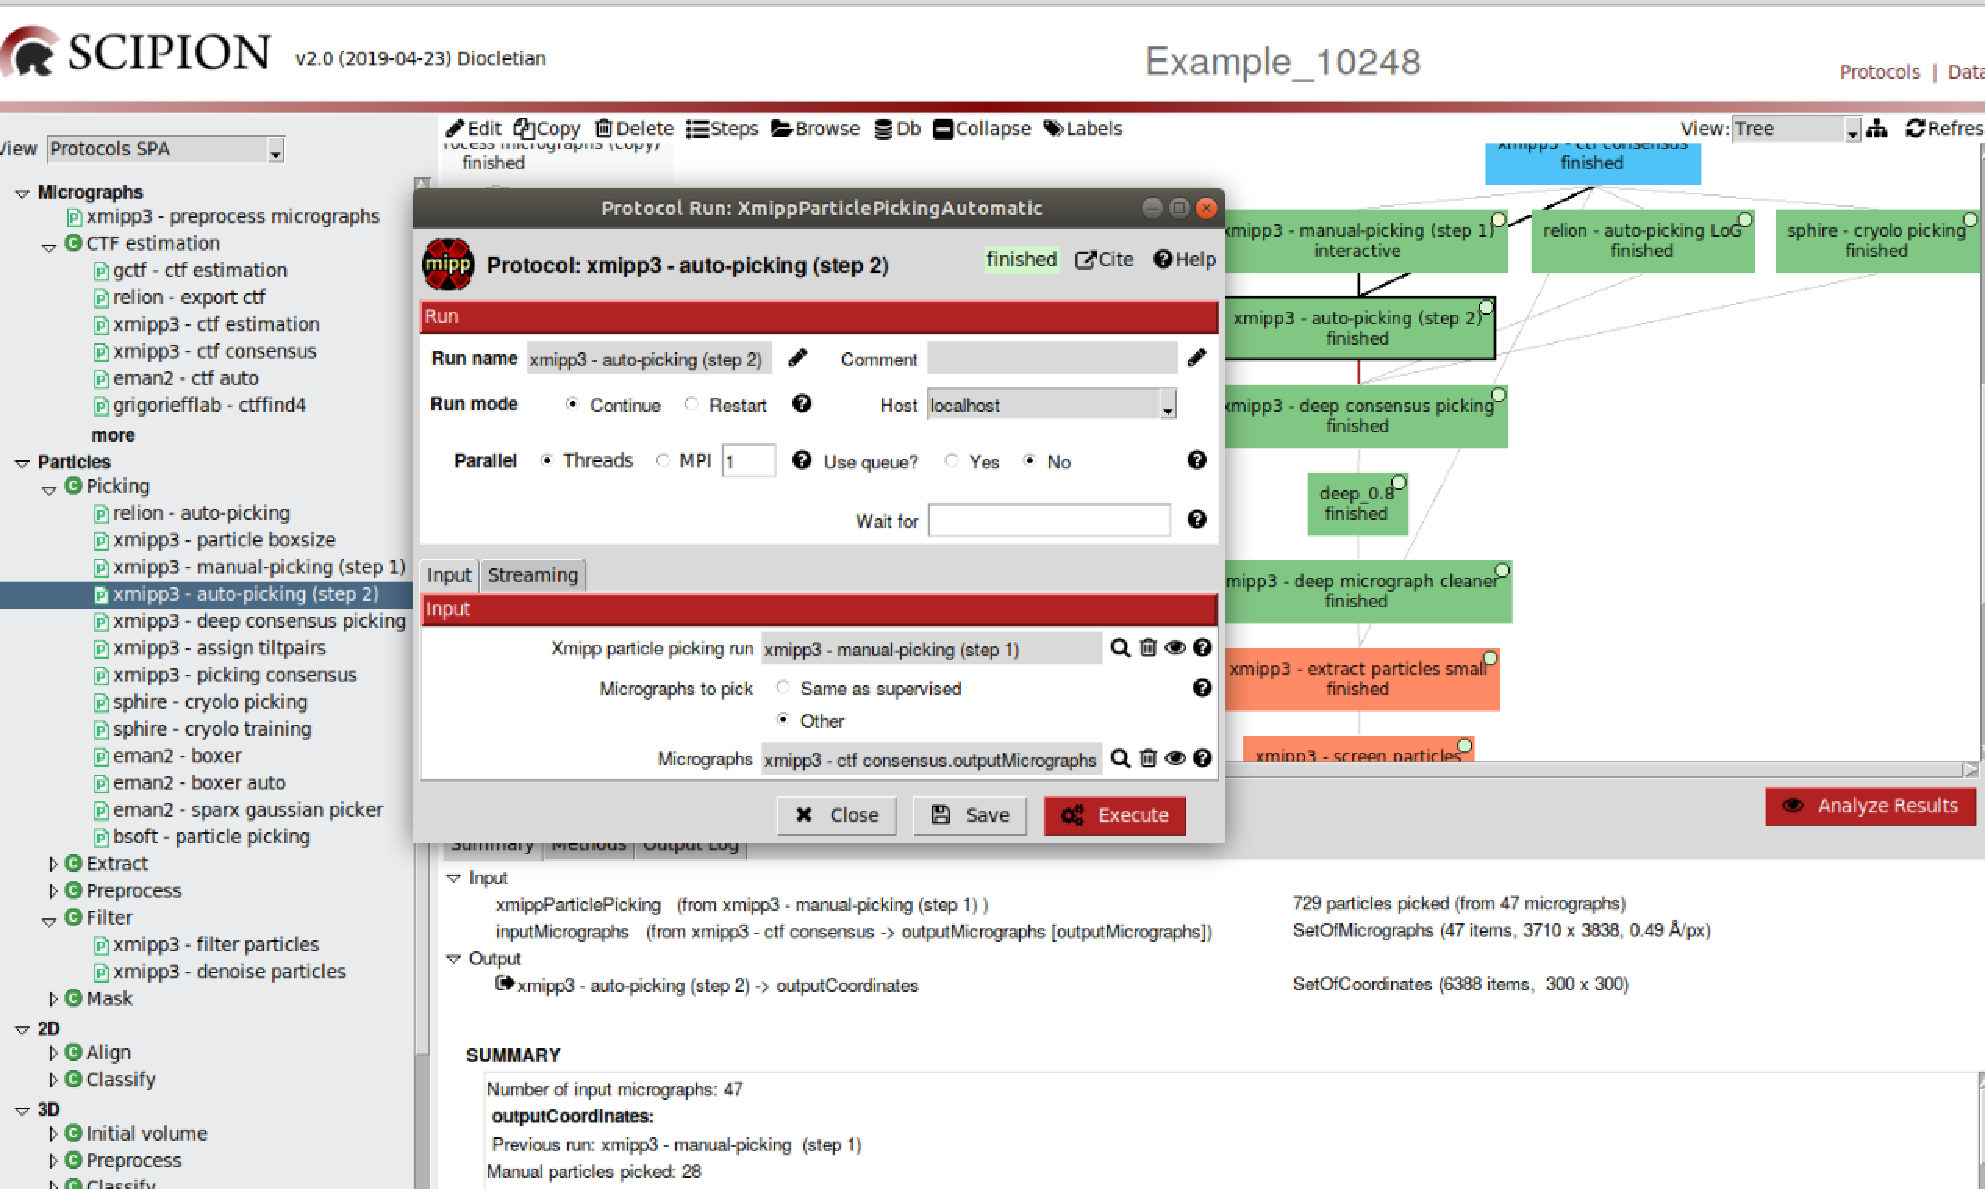
\includegraphics[width=0.95\textwidth]
  {{images/xmipp_autopicking_step2.pdf}}
  \caption{Completing the protocol \scommand{xmipp3- auto-picking (step 2)}.}
  \label{fig:xmipp_autopicking_step2}
  \end{figure}

  Results of all these protocols can be observed by pressing \scommand{Analyze Results}. In all cases a table details the number of particles extracted from each micrograph. Total number of particles appear in the lower part of this table, 6,233, 6,401, 748, and 6,607 running \scommand{relion- auto-picking LoG}, \scommand{sphire-cryolo picking}, \scommand{xmipp3- manual-picking (step1)}, and \scommand{xmipp3- auto-picking (step 2)}, respectively. As a conclusion, the three algorithms devoted to particle picking give us a similar result, around 6,500 particles. However, there are some differences among programs and we would like to keep only the coordinates of the good particles selected by the three methods.
  
  \subsection*{Consensus in particle picking}
  
  The protocol \scommand{xmipp3-deep consensus picking} (\ffigure{fig:xmipp_deep_consensus}) will try to select consensus particles among different particle picking algorithms. This protocol can also be used to get the consensus of sets of coordinates retrieved after using distinct setting of parameters with the same program. In our case, the whole sets of coordinates retrieved from the three previous methods have to be included as protocol input. 
  
  \begin{figure}[H]
  \centering
  \captionsetup{width=.8\linewidth} 
  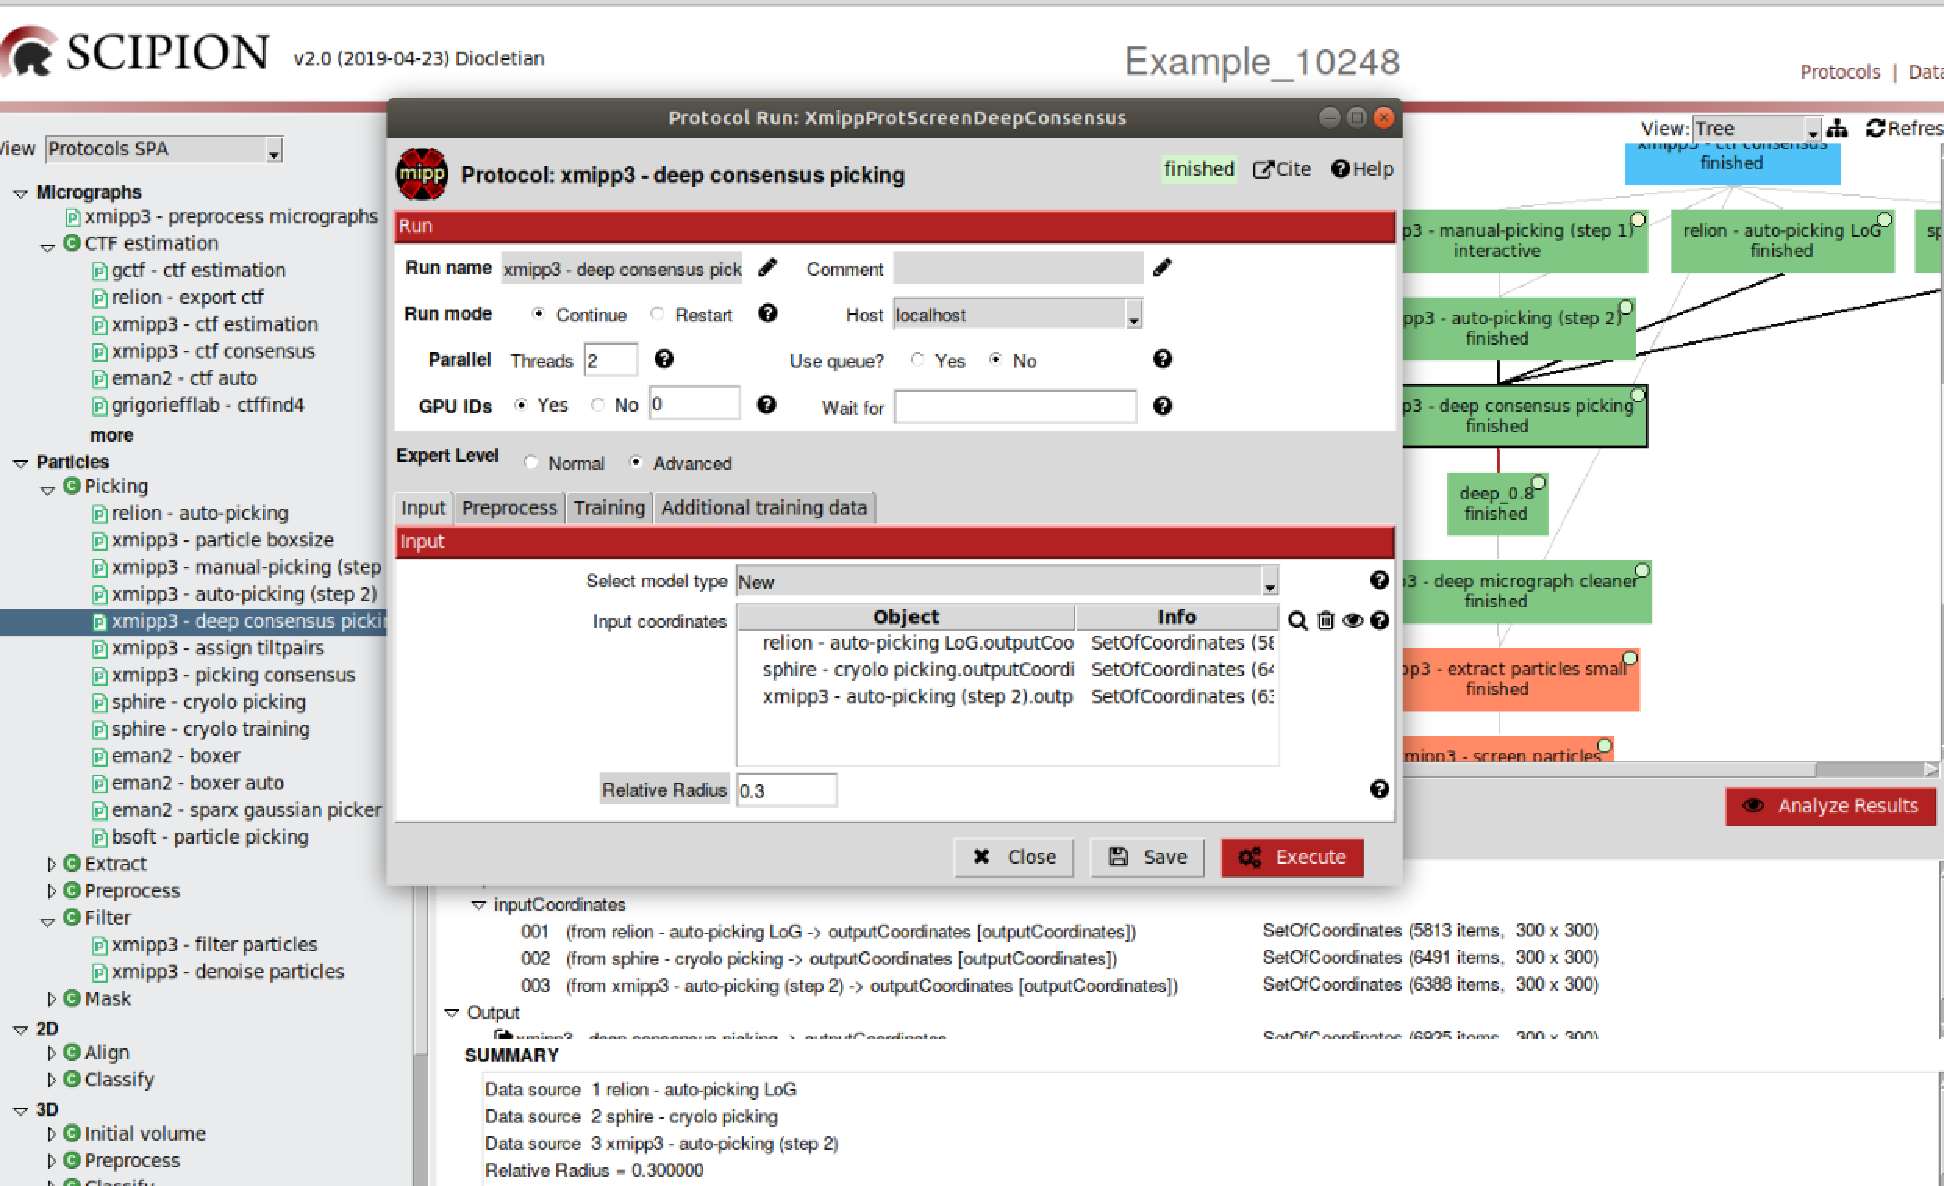
\includegraphics[width=0.95\textwidth]
  {{images/xmipp_deep_consensus.pdf}}
  \caption{Completing the protocol \scommand{xmipp3-deep consensus picking.}}
  \label{fig:xmipp_deep_consensus}
  \end{figure}
  
  A neural network will be trained with subsets of coordinates from particles picked and not picked. Finally, the method provides a score for each particle according to the neural network predictions. After pressing \scommand{Analyze Results}, a menu allows to visualize a table showing an image and the value of the deep learning score of all the particles (\ttt{Select particles/coordinates with high 'zScoreDeepLearning1' values}). Considering that bad particles show scores values close to 0.00 and good particles scores close to 1.00, the threshold, automatically set to 0.50, allows to select good particles. In our example, from the total number of particles (8,406), 1,671 particles will be rejected, and around 80\% of the total number of particles (6,735) will be selected. We have set, nevertheless, a more restricted threshold of 0.8. This way, 252 additional particles have been rejected and 6,483 particles still remain in the processing workflow.\\
  
  An additional cleaning step, accomplished with the protocol \scommand{xmipp3-deep micrograph cleaner}, removes particles located in carbon zones or in large impurities (\ffigure{fig:xmipp_deep_micrograph_cleaner}). Provide as input the previously selected set of coordinates and indicate the set of micrographs from which the computation will be performed. By default, we use the same as coordinates.
  
  \begin{figure}[H]
  \centering
  \captionsetup{width=.8\linewidth} 
  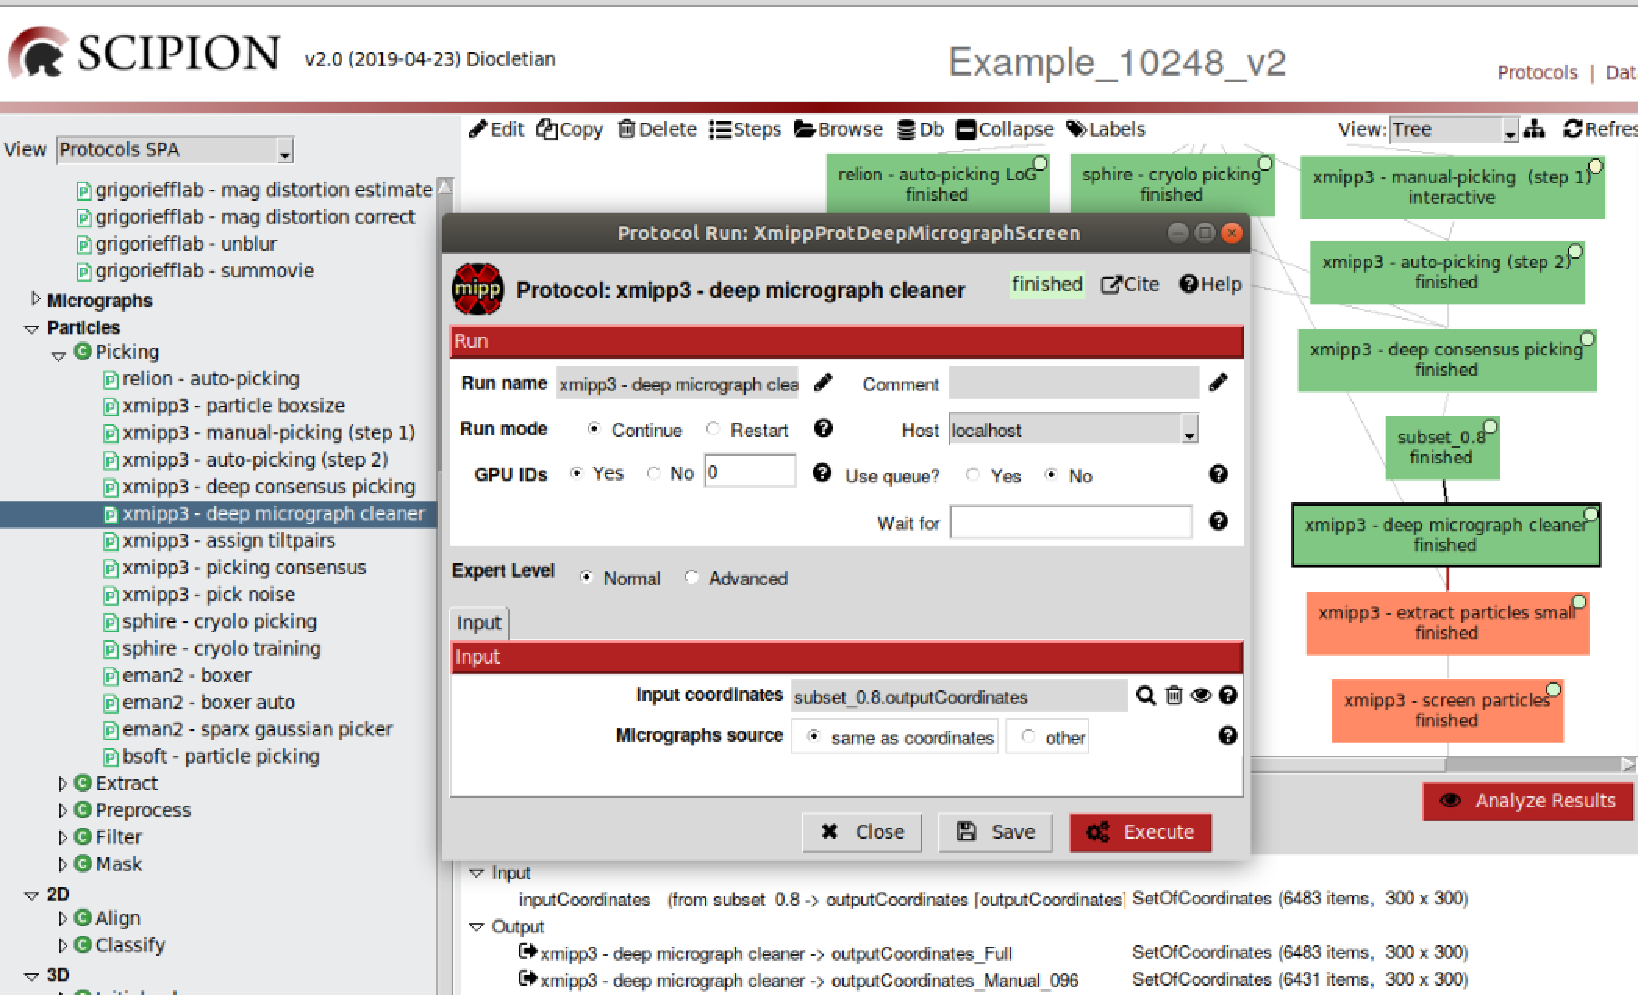
\includegraphics[width=0.95\textwidth]
  {images/xmipp_deep_micrograph_cleaner.pdf}
  \caption{Completing the protocol \scommand{xmipp3-deep consensus picking}.}
  \label{fig:xmipp_deep_micrograph_cleaner}
  \end{figure}
  
  After this additional step of cleaning, other set of 52 particles has been rejected. The coordinates of the remaining reliable 6,431 particles are selected for further processing.\\ 
